%!TEX TS-program = xelatex
%!TEX encoding = UTF-8 Unicode

%%%  Syllabus template for use with style files at http://kjhealy.github.com/latex-custom-kjh
%%%  Kieran Healy

\documentclass[11pt,article,oneside]{memoir}

% packages
\usepackage{org-preamble-xelatex} 

\AtBeginBibliography{\small}

% Definitions
\def\myauthor{Author}
\def\mytitle{Title}
\def\mycopyright{\myauthor}
\def\mykeywords{}
\def\mybibliostyle{plain}
\def\mybibliocommand{}
\def\mysubtitle{}
\def\myaffiliation{Louisiana State University}
\def\myaddress{100 Design}
\def\myemail{baharmon@lsu.edu} %harmon1@lsu.edu
\def\myweb{https://baharmon.github.io/}
\def\myphone{919.622.8414}
\def\myversion{}
\def\myrevision{}
\def\myaffiliation{\ \\Louisiana State University}
\def\myauthor{Brendan Harmon}
\def\mykeywords{Landscape Architecture, Syllabus, Graduate}
\def\mysubtitle{Syllabus}
\def\mytitle{{\normalsize \textsc{LA} 7032\newline} \huge \bfseries Geospatial modeling and fabrication}

\begin{document}

\setlength\bibitemsep{0.75em}

% fonts
\defaultfontfeatures{}
\defaultfontfeatures{Scale=MatchLowercase}         
\setmainfont[Scale=1, Path = fonts/lato/,BoldItalicFont=Lato-RegIta,BoldFont=Lato-Reg,ItalicFont=Lato-LigIta]{Lato-Lig}
\setsansfont[Scale=1, Path = fonts/lato/,BoldItalicFont=Lato-RegIta,BoldFont=Lato-Reg,ItalicFont=Lato-LigIta]{Lato-Lig}
\setmonofont[Mapping=tex-text,Scale=0.8,Path = fonts/inconsolata/]{i}

\def\ind{\hangindent=1 true cm\hangafter=1 \noindent}
\def\labelitemi{$\cdot$}
\chapterstyle{article-4-sans}  
\title{\LARGE \mytitle}     
\author{\Large\myauthor \newline \footnotesize\texttt{\noindent\myemail}}
\date{Fall 2017. Design 217.\newline Tuesday \& Thursday 1:30am--5:20pm.}
\published{\,}

\maketitle

% -------------------------------- COVER PAGE -------------------------------- 

% full-page, 30% opacity greyscale image
% with cast metal model dissolving to point cloud (plas.io)

% -------------------------------- DESCRIPTION -------------------------------- 

\section{Course Description}

This course is an introduction to digital design for landscape architects. 
%
In this course you will develop a creative digital design process 
seamlessly integrating research and design
using geographic information systems (GIS),
3D modeling and rendering, and
visual programming. 
%
You will learn how to use geospatial data 
to model and analyze landscapes
and visual programming to 
parametrically model and transform new landforms. 
%
You will learn how to model plants -- from trees to grasses -- in 3D, 
automatically distribute them across your digital landscape,
and render photorealistic scenes. 
%
Each week you will spend a day in a workshop
learning new methods
and a day developing your projects.\\

\noindent In preparation for this course please read:
%
\nocite{*} \printbibliography[keyword=intro, heading=none]

%\begin{figure}
%    \begin{center}
%        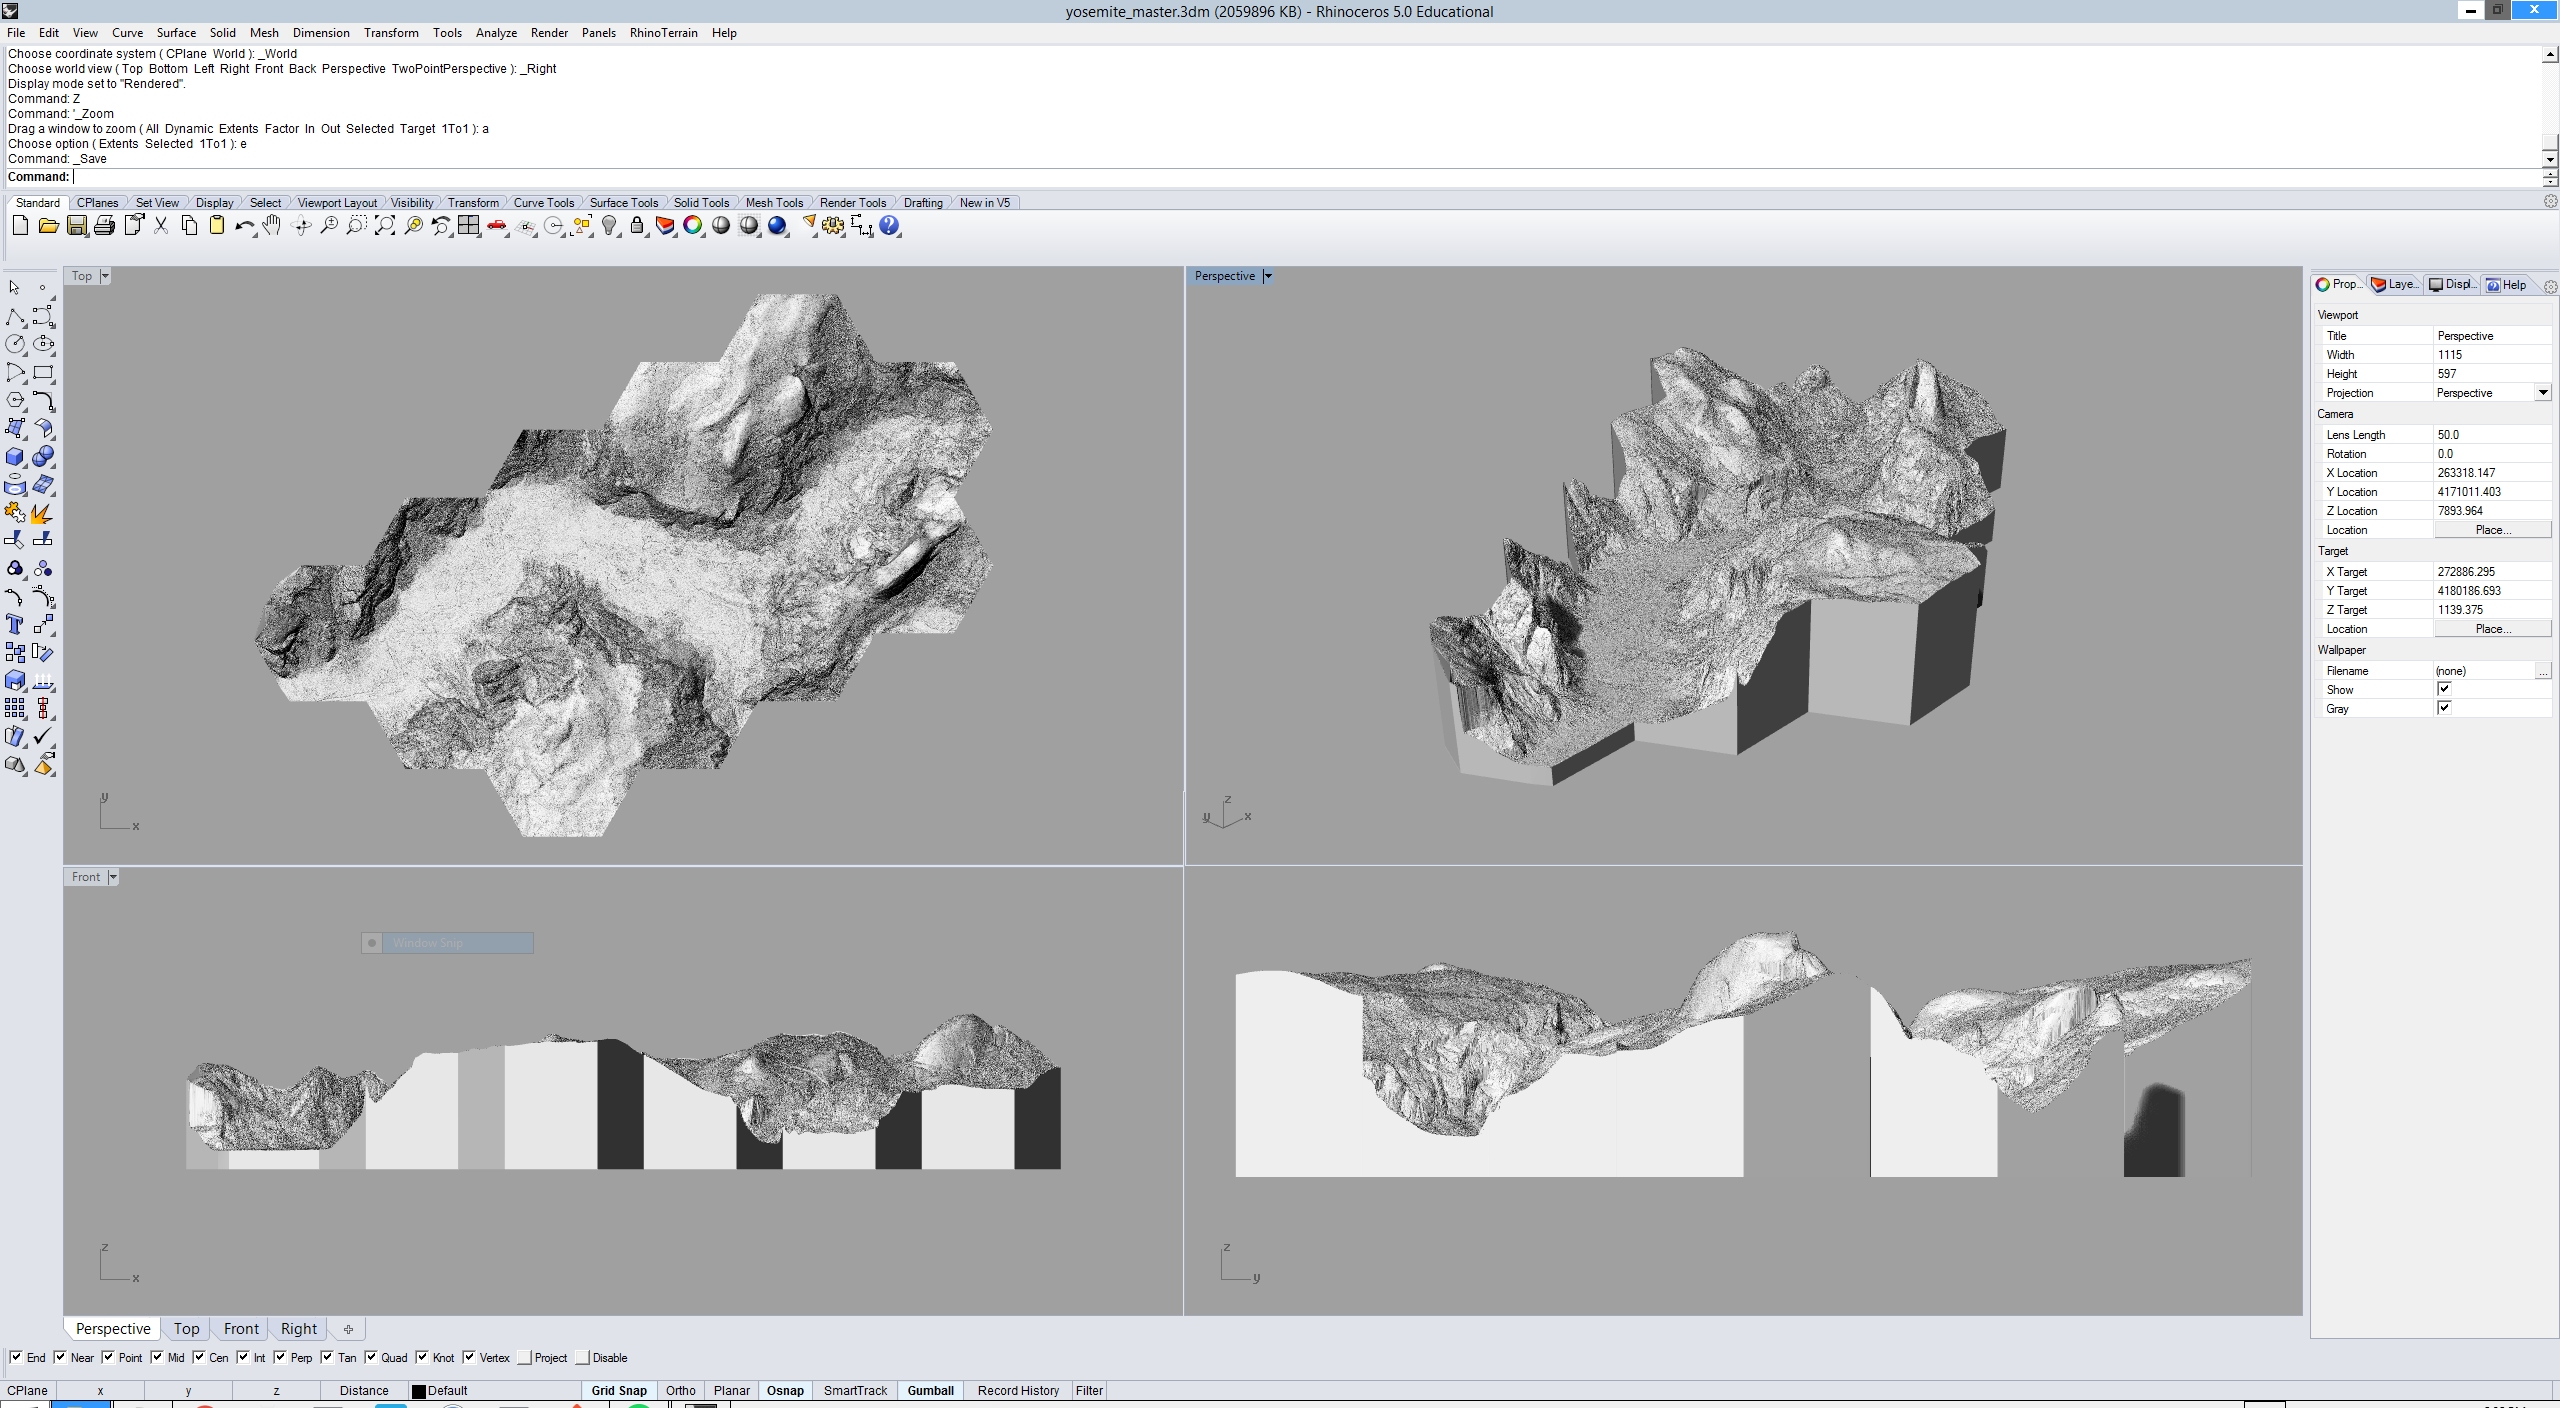
\includegraphics[width=\textwidth]{images/yosemite_1.png}
%        \caption{...}
%        \label{fig:yosemite}
%    \end{center}
%\end{figure}

%\clearpage

% -------------------------------- SCHEDULE -------------------------------- 
\section{Course Schedule}

\begin{table}[H]
\small
\begin{tabular}{l l @{\hskip 1cm}l}
%
\textbf{1} & Terrain modeling\\
\textbf{2} & Digital fabrication & \textbf{Workshop:} Lost foam casting\\
\textbf{3} & Geospatial analysis\\
\textbf{4} & Geospatial simulation & \textbf{Project:} Geospatial modeling\\
%
\textbf{5} & Surface modeling\\
\textbf{6} & Visual programming\\
\textbf{7} & Families of form\\
\textbf{8} & Generative processes & \textbf{Project:} Generative design\\
%
\textbf{9} & Image classification\\
\textbf{10} & 3D plants\\
\textbf{11} & Particle systems\\
\textbf{12} & Rendering\\
\textbf{13} & Physics\\
\textbf{14} & Exhibition & \textbf{Project:} Ecosystem modeling\\
%
\end{tabular}
\end{table}

%\clearpage

% -------------------------------- Project -------------------------------- 
\section{Projects}
Through a series of 3D modeling projects you will 
study how to restore a highly eroded landscape with a deep gully.
You will work in small teams and present an exhibition of your
models and renderings at the end of the course.\\

% Exhibition: project simulations over wall-mounted models

\noindent \textbf{Geospatial modeling}
Using lidar data you will model, analyze, and digitally fabricate
the topography of the study landscape. 
%
%After processing the lidar point cloud
%and generating digital models of the topography,
Each group will CNC mill a physical model of the landscape
in a different media -- either medium density fiberboard, 
polystyrene foam, or urethane foam.
Then each group will prepare a different set of 
-- either topographic, hydrologic, or sedimentation -- 
analyses and simulations.\\

% Topographic: contours, slope, hillshade, landforms
% Hydrologic: watershed, flow accumulation, water flow
% Sedimentation: sediment flux, erosion-deposition, landscape evolution

\noindent \textbf{Generative design}
Using visual programming you will generatively design
erosion control features to restore your degraded study landscape.
Through a series of algorithmically generated design interventions 
you will explore interactions between 
topographic form and hydrologic processes.
Your goal is to catalyze topographic changes that will 
restore the landscape to a dynamic equilibrium.  
You will produce 3D printed models of your designs
and augment these with projected water flow and sediment flux. \\

\noindent \textbf{Ecosystem modeling}
After mapping the existing vegetation 
you will design, model, and render in 3D
a planting plan to restore this degraded landscape. 
You will produce beautiful, photorealistic 3D renderings  
of the existing landscape and your design. \\

%\clearpage

% -------------------------------- SESSIONS -------------------------------- 
\section{Sessions}

\renewcommand*{\bibfont}{\footnotesize}

\noindent \textbf{Terrain modeling}
Model topography in 3D from lidar data.\\

\noindent \textbf{Digital fabrication}
Use computer numerical control (CNC) machining 
to carve physical models of topography. 
Learn how to cast a topographic model
in aluminum.
%
\nocite{*} \printbibliography[keyword=fabrication, heading=none]
\vspace*{0.5em}

%\noindent \textbf{Workshop | Lost foam casting}
%In this workshop learn how to cast a topographic model
%in aluminum using a CNC milled foam form.\\

\noindent \textbf{Geospatial analysis}
Model and analyze topographic parameters including 
contours, slope, hillshading, and landforms
and hydrologic parameters 
including watersheds and flow accumulation. \\

\noindent \textbf{Geospatial simulation}
Simulate the physical processes that shape landscapes including
water flow, sediment flux, erosion-deposition, and landscape evolution.\\

\noindent \textbf{Surface modeling}
Model complex, continuous, 3D surfaces 
using non-uniform rational basis splines (NURBS).\\

\noindent \textbf{Visual programming}
Use visual programming to automatically generate
patterns and forms.
%
\nocite{*} \printbibliography[keyword=algorithmic, heading=none]
\vspace*{0.5em}

\noindent \textbf{Families of form}
Use visual programming to procedurally generate families of form
based on parametric variations.
%
\nocite{*} \printbibliography[keyword=procedural, heading=none]
\vspace*{0.5em}

\noindent \textbf{Generative processes}
Procedurally generate dynamic forms using 
parametric equations and attractors.\\

\noindent \textbf{Image classification}
Use aerial photography to automatically classify 
different types of landcover.\\

\noindent \textbf{3D plants}
Procedurally model unique specimens 
of trees and other plants in 3D.
Model an ecosystem in 3D using 3D plant libraries.
%
\nocite{*} \printbibliography[keyword=plants, heading=none]
\vspace*{0.5em}

\noindent \textbf{Particle systems}
Generate fields of plants 
using particle systems. \\

\noindent \textbf{Rendering}
Setup lights, prepare materials and textures, 
and render 3D scenes with raytracing.\\

\noindent \textbf{Physics}
Simulate processes like water flow and rock fall
using a physics engine.\\

\noindent \textbf{Exhibition}
Present your work in a gallery style exhibition.\\

%\clearpage

% -------------------------------- Software -------------------------------- 
\section{Software}
GRASS GIS | \url{https://grass.osgeo.org/} \\
Rhinoceros | \url{https://www.rhino3d.com/}\\
RhinoTerrain | \url{http://www.rhinoterrain.com/}\\
RhinoCAM | \url{https://mecsoft.com/rhinocam-software/}\\
Grasshopper | \url{http://grasshopper3d.com/}\\
Blender | \url{https://www.blender.org/}\\

% -------------------------------- Resources -------------------------------- 
\section{Resources}
Intro to GRASS GIS | \url{https://ncsu-geoforall-lab.github.io/grass-intro-workshop/}\\
Hydrology in GRASS GIS | \url{https://grasswiki.osgeo.org/wiki/Hydrological_Sciences}\\
Grasshopper Primer | \url{http://grasshopperprimer.com}\\
BlenderGIS tutorial | \url{https://github.com/ptabriz/ICC_2017_Workshop}

%% -------------------------------- Supplies --------------------------------  
%\section{Supplies}
%Alcohol-based markers | \emph{Chartpak or Copic}\\
%Felt-tip markers | \emph{Tombow Dual Brush Pens or Pentel Sign Pen}\\
%Trace | \emph{White or Canary}\\
%Polymer enriched sand | \emph{Kinetic Sand, 11~lbs}\\
%Medium density fiberboard \\

\clearpage

%% -------------------------------- Required readings -------------------------------- 
%\section{Required books}
%\renewcommand*{\bibfont}{\normalsize} %\small
%\vspace*{0.5cm}
%\nocite{*}
%\setlength\bibitemsep{1\baselineskip}
%\printbibliography[keyword=required, heading=none]

% -------------------------------- Readings -------------------------------- 
\section{Readings}
\renewcommand*{\bibfont}{\normalsize} %\small
\vspace*{0.5cm}
\nocite{*}
\setlength\bibitemsep{1\baselineskip}
\printbibliography[heading=none]

\clearpage

% -------------------------------- Policies -------------------------------- 
\section{Policies}

\noindent \textbf{Time Commitment Expectations}
LSU's general policy states that for each credit hour, you (the student) should plan to
spend at least two hours working on course related activities outside of class. Since this course is for three credit hours, you should expect to spend a minimum of six hours outside of class each week working on assignments for this course. For more information see: 
\url{http://catalog.lsu.edu/content.php?catoid=12&navoid=822}.\\

\noindent \textbf{LSU student code of conduct}
The LSU student code of conduct explains student rights, excused absences, and what is expected of student behavior. Students are expected to understand this code:  \url{http://students.lsu.edu/saa/students/code}.\\ %Any violations of the LSU student code will be duly reported to the Dean of Students.\\

\noindent \textbf{Disability Code}
The University is committed to making reasonable efforts to assist individuals with disabilities in
their efforts to avail themselves of services and programs offered by the University. To this end,
Louisiana State University will provide reasonable accommodations for persons with
documented qualifying disabilities. If you have a disability and feel you need accommodations in
this course, you must present a letter to me from Disability Services in 115 Johnston Hall,
indicating the existence of a disability and the suggested accommodations.\\

\noindent \textbf{Academic Integrity}
According to section 10.1 of the LSU Code of Student Conduct, ``A student may be charged with Academic Misconduct'' for a variety of offenses, including the following: unauthorized copying, collusion, or collaboration; ``falsifying'' data or citations; ``assisting someone in the commission or attempted commission of an offense''; and plagiarism, which is defined in section 10.1.H as a ``lack of appropriate citation, or the unacknowledged inclusion of someone else's words, structure, ideas, or data; failure to identify a source, or the submission of essentially the same work for two assignments without permission of the instructor(s).''\\

\noindent \textbf{Plagiarism and Citation Method}
Plagiarism is the ``lack of appropriate citation, or the unacknowledged inclusion of someone else's words, structure, ideas, or data; failure to identify a source, or the submission of essentially the same work for two assignments without permission of the instructor(s)'' (Sec. 10.1.H of the LSU Code of Student Conduct). As a student at LSU, it is your responsibility to refrain from plagiarizing the academic property of another and to utilize appropriate citation method for all coursework. In this class, it is recommended that you use Chicago Style author-date citations. Ignorance of the citation method is not an excuse for academic misconduct. 

\noindent \textbf{Graduate Certificate in GIS}
This course counts as an applied topics course for the 
Graduate Certificate in Geographic Information Science.
The Graduate Certificate in Geographic Information Science at LSU 
is a 12 credit hour standalone certificate with courses offered 
in the Department of Geography and Anthropology, College of Art and Design, 
Department of Economics, School of the Coast and Environment, 
Department of Civil and Environmental Engineering, 
and Department of Computer Science. 
For more information about the Graduate Certificate in GIS visit: 
\url{http://ga.lsu.edu/gis-certificate/}.

%\noindent \textbf{Communication Intensive}
%This is a certified Communication-Intensive (C-I) course,
%which meets all of the requirements set
%forth by LSU’s Communication across the Curriculum program, including
%\begin{itemize}
%\item instruction and assignments emphasizing 
%informal and formal visual and technological communication,
%\item teaching of discipline-specific communication techniques,
%\item use of feedback loops for learning,
%\item 40\% of the course grade rooted in communication-based work, and
%\item practice of ethical and professional work standards.
%\end{itemize}
%Students interested in pursuing the LSU Distinguished Communicators 
%certification may use this C-I course for credit. 
%For more information about this student recognition program visit: 
%\url{www.cxc.lsu.edu}.

\end{document}
